% Concept paper based on the supplied cs-techrep example template.
% Language: American English (the class maps 'english' to en-US).
% Verify institutional department and report metadata before submission.
\PassOptionsToPackage{type=CC,modifier=by,version=4.0}{doclicense}
\documentclass[conference,a4paper,flushend]{cs-techrep}
\pdfoutput=1

% The supplied class configures biblatex/biber and the IEEE-style layout.
% Shorten long author lists in bibliography without altering the document layout.
\AtBeginDocument{\ExecuteBibliographyOptions{maxbibnames=4,minbibnames=1}}
\addbibresource{references.bib}

\cstechrepAuthorListTex{Timo Gr\"af, Maria Lyoteva, Dominik Schwagerl, and Tsvetan Stanchev}
\cstechrepAuthorListBib{\detokenize{Gr\"af}, Timo and Lyoteva, Maria and Schwagerl, Dominik and Stanchev, Tsvetan}
\cstechrepTitleTex{MergeLens: Predicting Pull Request Outcomes from Titles and Descriptions}
\cstechrepTitleBib{{MergeLens}: Predicting Pull Request Outcomes from Titles and Descriptions}
\cstechrepDepartment{Department of Electrical Engineering, Media, and Computer Science}
\cstechrepInstitution{Ostbayerische Technische Hochschule Amberg-Weiden}
\cstechrepAddress{Amberg, Germany}
\cstechrepType{Concept Paper}
\cstechrepYear{2026}
\cstechrepMonth{11}
\cstechrepNumber{Draft}
\cstechrepLang{english}
% Use an explicit month for this draft so the report's self-reference
% does not occupy a bibliography number reserved for related work.
\IEEEspecialpapernotice{\cstechrepType: \cstechrepNumber, November \cstechrepYear}

% Required by the provided class/template for the report's self-reference.
\filecontentsForceExpansion|[]
\begin{filecontents*}[overwrite]{selfref.bib}
@TECHREPORT{selfref,
  author = {|cstechrepAuthorListBib},
  title = {\cstechrepTitleBib},
  institution = {\cstechrepInstitution, \cstechrepDepartment},
  type = {\cstechrepType},
  number = {\cstechrepNumber},
  year = {|cstechrepYear},
  month = {|cstechrepMonth},
  langid = {|cstechrepLang},
}
\end{filecontents*}

% The template self-citation otherwise consumes reference number [1]; keep
% the prescribed license notice without citing the draft as prior work.
\makeatletter
\renewcommand{\mycopyrightnotice}{{\footnotesize
  \begin{minipage}{0.8\textwidth}\centering
    \href{\doclicenseURL}{\doclicenseIcon{} This work is licensed under a
    \doclicenseLongNameRef{} (\doclicenseNameRef{}) license.}
  \end{minipage}}}
\makeatother

\usepackage{tikz}
\usetikzlibrary{arrows.meta,positioning,fit,backgrounds}
\usepackage{enumitem}

% Compact, consistent requirement formatting, preserving the template's US convention.
\setlist[enumerate,1]{leftmargin=*,itemsep=2.4pt,topsep=3pt,parsep=0pt}
\setlist[itemize]{leftmargin=1.25em,topsep=1pt,itemsep=1pt,parsep=0pt}

\begin{document}
\selectlanguage{\cstechrepLang}
\maketitle

\begin{abstract}
Maintainers of active GitHub repositories must assess numerous pull requests (PRs), including proposals of uncertain value. \emph{MergeLens} investigates whether a compact, fine-tuned language model can provide an early indication of a PR's potential usefulness using only its English title and description. Historical GH Archive events will supply labeled examples based on observed merge outcomes. The proposed system comprises a reproducible data-processing and training pipeline, a containerized inference service, and a web interface for maintainer-triggered predictions. Its predictive value will be assessed on held-out data; it is intended to support, not replace, human review.
\end{abstract}

\begin{IEEEkeywords}
pull requests, GitHub, GH Archive, text classification, fine-tuning, maintainer support.
\end{IEEEkeywords}

\section{Introduction and Motivation}
Popular open-source repositories may receive more pull requests (PRs) than their maintainers can promptly review. Each proposal requires an assessment of its relevance, technical contribution, and fit with the project's goals. AI-assisted coding tools can make it easier to submit contributions, including superficially plausible proposals that offer limited value. This increases the importance of efficient initial triage, particularly when maintainers have limited time \cite{baltes2026aislop}.

A comprehensive code-based assessment can be costly: inspecting large changes and their repository context may require substantial input context and computational resources. Generic language models are also not specifically trained to estimate PR acceptance. \emph{MergeLens} therefore explores a deliberately narrower approach: can the language of a PR title and description alone provide a useful first indication of whether its proposed change is likely to benefit a project? A potentially useful PR is understood here as a contribution that fixes a problem, improves an existing technical property, or introduces a relevant functional enhancement.

The system will learn from historical GitHub PRs available through GH Archive \cite{gharchive}, using a merge as a positive training label and closure without merging as a negative label. This large-scale approximation is a practical learning signal, not a definitive measure of technical merit. The objective is to evaluate whether a relatively compact, specialized model can help maintainers prioritize manual reviews without analyzing source code or making acceptance decisions on their behalf.

\section{Related Work}
Chen et al.'s \emph{E-PRedictor} predicts PR acceptance at submission time by combining BERT-derived representations of PR descriptions and code changes with contributor, PR, and project features \cite{chen2025epredictor}. Similarly, \emph{CTCPPre} uses textual, code, contributor, and project characteristics to predict acceptance \cite{jiang2020ctcppre}. Both demonstrate the established relevance of acceptance prediction but rely on information beyond PR text. Pirouzkhah et al. found associations between specific elements of PR descriptions and review outcomes, including merge decisions \cite{pirouzkhah2026descriptions}. Building on this research, the proposed experiment isolates the predictive information in the \emph{title and description} and studies its usefulness with a fine-tuned, lightweight classifier rather than a feature-rich, code-aware system.

\section{Functional Design}
The architecture in Fig.~\ref{fig:architecture} separates an offline learning pipeline from the online maintainer workflow. A data engineer prepares labeled historical examples; a model developer trains and evaluates the classifier; a repository maintainer views a PR retrieved via GitHub API or webhooks \cite{githubpullapi} and requests an indication of its likely merge outcome. The database retains both extracted records and processed datasets. Optional account-based navigation and contributor metadata are outside the initial pipeline.

\begin{figure}[t]
  \centering
  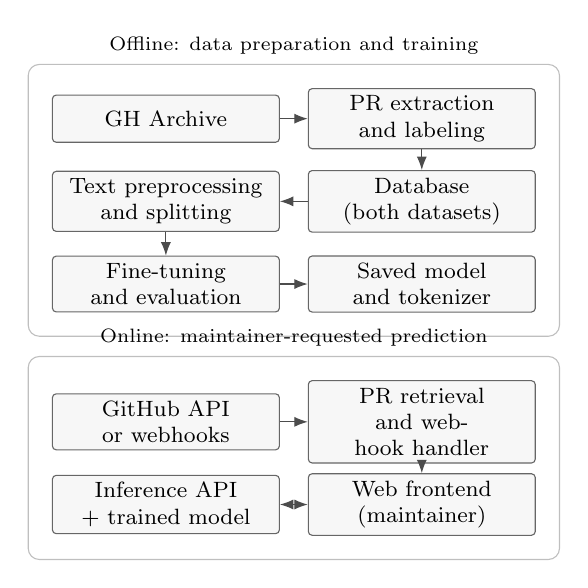
\begin{tikzpicture}[
      font=\footnotesize,
      box/.style={draw=black!60,rounded corners=1.4pt,fill=black!3,align=center,
        minimum height=6mm,text width=27mm,inner sep=2.6pt},
      arr/.style={-{Latex[length=1.7mm]},thin,draw=black!70},
      both/.style={{Latex[length=1.7mm]}-{Latex[length=1.7mm]},thin,draw=black!70},
    ]
    % Offline batch processing and model development (serpentine order).
    \node[box] (archive) at (0,0) {GH Archive};
    \node[box] (extract) at (3.25,0) {PR extraction\\and labeling};
    \node[box] (db) at (3.25,-1.05) {Database\\(both datasets)};
    \node[box] (prep) at (0,-1.05) {Text preprocessing\\and splitting};
    \node[box] (train) at (0,-2.10) {Fine-tuning\\and evaluation};
    \node[box] (model) at (3.25,-2.10) {Saved model\\and tokenizer};
    \draw[arr] (archive) -- (extract);
    \draw[arr] (extract) -- (db);
    \draw[arr] (db) -- (prep);
    \draw[arr] (prep) -- (train);
    \draw[arr] (train) -- (model);
    \node[draw=black!25,rounded corners,fit=(archive)(extract)(db)(prep)(train)(model),
      inner sep=3mm,label={[font=\scriptsize]above:Offline: data preparation and training}] {};

    % Online workflow: webhooks are received by backend integration, not by browser.
    \node[box] (github) at (0,-3.85) {GitHub API\\or webhooks};
    \node[box] (adapter) at (3.25,-3.85) {PR retrieval\\and webhook handler};
    \node[box] (ui) at (3.25,-4.90) {Web frontend\\(maintainer)};
    \node[box] (api) at (0,-4.90) {Inference API\\+ trained model};
    \draw[arr] (github) -- (adapter);
    \draw[arr] (adapter) -- (ui);
    \draw[both] (ui) -- (api);
    \node[draw=black!25,rounded corners,fit=(github)(adapter)(ui)(api),
      inner sep=3mm,label={[font=\scriptsize]above:Online: maintainer-requested prediction}] {};
  \end{tikzpicture}
  \caption{Proposed offline training and online PR assessment. Preprocessed datasets are written back to the database; the saved model is loaded by the inference API.}
  \label{fig:architecture}
\end{figure}

\section{Functional Requirements: User Stories}
The following user stories define the minimum viable product (MUST), desirable enhancements (SHOULD), optional extensions (COULD), and explicit exclusions (WON'T). A PR's \emph{outcome} refers to its historically observed merged or closed-without-merge status.

\subsection{MUST}
\begin{enumerate}[label={US\arabic*},series=stories]
\item \textbf{Acquire and Label PRs.} As a data engineer, I want to extract PR-related events from GH Archive so that historical training examples can be labeled.
  \begin{itemize}
    \item \textbf{Acceptance:} Given archive files for a selected period, when extraction runs, then PR identifiers, titles, descriptions, and determinable terminal outcomes are collected; unrelated events are excluded and repeated events are associated with the same PR.
  \end{itemize}

\item \textbf{Persist Project Data.} As a data engineer, I want extracted and prepared PR records stored in a database so that downstream steps can retrieve them reliably.
  \begin{itemize}
    \item \textbf{Acceptance:} Given an extracted or processed record, when it is stored, then it can be retrieved for the corresponding next processing stage.
  \end{itemize}

\item \textbf{Prepare and Split Data.} As a model developer, I want standardized English PR text and separate datasets so that training and evaluation use consistent inputs.
  \begin{itemize}
    \item \textbf{Acceptance:} Given stored records, when preprocessing completes, then unusable records are filtered, text is normalized, English entries are selected, and train/validation/test sets are persisted without PR overlap.
  \end{itemize}

\item \textbf{Fine-Tune a Binary Classifier.} As a model developer, I want to adapt a pretrained language model so that it can predict PR merge outcomes from title and description alone.
  \begin{itemize}
    \item \textbf{Acceptance:} Given the training split, when training completes, then the model uses a two-output classification head and produces a saved model artifact and tokenizer for inference.
  \end{itemize}

\item \textbf{Evaluate Generalization.} As a model developer, I want performance measured on unseen PRs so that the value of the text-only approach can be assessed.
  \begin{itemize}
    \item \textbf{Acceptance:} Given nonoverlapping validation and test sets, when evaluation runs, then per-class precision, recall, F1, and a confusion matrix are reported; the test set is not used for training.
  \end{itemize}

\item \textbf{Request and View PR Assessment.} As a maintainer, I want to view a PR retrieved through the GitHub API or a webhook and trigger a prediction so that I can prioritize my review.
  \begin{itemize}
    \item \textbf{Acceptance:} Given a retrievable PR, when I open the view, then its title and description are displayed; when I select \emph{Evaluate}, the frontend calls the inference API and displays a prediction or an actionable error.
  \end{itemize}

\item \textbf{Run Integrated Modules.} As a developer, I want the project's modules containerized so that the data workflows, database, model service, and frontend can be integrated reproducibly.
  \begin{itemize}
    \item \textbf{Acceptance:} Given the documented Docker configuration, when the required services are started, then the components connect and a sample PR evaluation reaches the inference service.
  \end{itemize}
\end{enumerate}

\subsection{SHOULD}
\begin{enumerate}[label={US\arabic*},resume=stories]
\item \textbf{Display a Prediction Score.} As a maintainer, I want a clearly labeled model-derived score alongside the predicted class so that I can judge the strength of the initial indication.
  \begin{itemize}
    \item \textbf{Acceptance:} Given a successful inference, the UI shows the predicted class and a clearly labeled score without presenting it as proof of PR quality.
  \end{itemize}
\end{enumerate}

\subsection{COULD}
\begin{enumerate}[label={US\arabic*},resume=stories]
\item \textbf{Browse PRs Through GitHub Login.} As a maintainer, I want to sign in with GitHub, list open PRs for an accessible repository, and select one for evaluation.
  \begin{itemize}
    \item \textbf{Acceptance:} After authorization, selecting a listed PR displays its title and description and enables the same evaluation action as in US6.
  \end{itemize}
\item \textbf{Compare Additional Contributor Features.} As a model developer, I want to include contributor metadata, such as account age or commit history, so that I can test whether it improves predictive performance.
  \begin{itemize}
    \item \textbf{Acceptance:} If implemented, the acquisition, preprocessing, and model pipelines support the added features, and evaluation compares them with the title-and-description baseline.
  \end{itemize}
\end{enumerate}

\subsection{WON'T (MVP)}
The system will neither autonomously accept/reject PRs nor inspect complete code changes for its initial prediction. Mandatory cloud hosting is also outside the MVP scope.

\section{Non-Functional Requirements}
\textbf{Scalability and reliability:} Historical archives should be processed incrementally without loading the entire corpus into memory; failed jobs should be restartable without duplicating PR records. \textbf{Reproducibility:} Dataset splits, preprocessing choices, model settings, and evaluation outputs should be traceable to a run and model version. \textbf{Usability and performance:} Predictions and failures must be presented clearly; inference latency should be measured on the target local hardware. \textbf{Security:} The MVP uses publicly accessible PR data; any future GitHub authentication must protect access tokens and request only necessary permissions.

\section{Technical Key Components and Technology Stack}
The proposed pipeline uses \textbf{Python} for GH Archive ingestion and PR extraction. \textbf{Polars} \cite{polarsdocs} is a candidate for memory-efficient, single-machine batch processing; \textbf{PySpark} \cite{zaharia2016spark} remains an option if the selected observation period and available infrastructure justify distributed execution. A \textbf{PostgreSQL} database \cite{postgresdocs} is under consideration for structured PR records and both raw-extracted and prepared datasets; its schema is not yet fixed.

Model development will likely use \textbf{PyTorch} \cite{paszke2019pytorch} and \textbf{Hugging Face Transformers} \cite{wolf2020transformers}. A compact \textbf{BERT-based encoder} \cite{devlin2019bert} with a two-logit classification head is a candidate, not a final selection. \textbf{scikit-learn} \cite{pedregosa2011sklearn} may support metrics and a simple baseline. For deployment, a \textbf{FastAPI} service \cite{fastapidocs} will load the saved model and tokenizer and expose inference to a prospective \textbf{React/TypeScript} frontend \cite{reactdocs,typescriptdocs}. \textbf{Docker} \cite{merkel2014docker}, potentially coordinated with \textbf{Docker Compose} \cite{composedocs}, will support local execution; a public cloud service is not required. Basic CI with \textbf{GitHub Actions} \cite{githubactionsdocs} may be considered.

The main design trade-off is lower inference input size and simpler integration versus missing code and repository context. Practical risks include variable archive payloads, class imbalance, labeling noise, GitHub API limits, and fine-tuning cost. The training texts should reflect information available when a PR is submitted, avoiding outcome-related leakage; a simple text baseline may be used for comparison. Observation period, model size, compute budget, and final deployment configuration will be chosen during implementation.

\section{Conclusion and Outlook}
\emph{MergeLens} proposes a text-only, early PR triage indicator built from historical GitHub outcomes. Its central experiment is whether title and description carry enough signal for useful predictions with a compact fine-tuned model. A separate test set will establish the approach's limitations before any claim of practical benefit. Optional GitHub sign-in and contributor metadata may broaden usability and predictive context if resources permit; maintainer judgment remains authoritative.

\printbibliography[notcategory=selfref,resetnumbers=true,heading=bibintoc,title={References}]
\end{document}
